\documentclass[12pt]{article}
% Chinese Support
\usepackage{xeCJK}
\setCJKmainfont{STSong}
% \setmainfont{Times New Roman}

\usepackage{float}

% for symbol
\usepackage{gensymb}
% matrix
\usepackage{amsmath}

% For images
\usepackage{graphicx}
\graphicspath{ {./screenshoot/} }

\newcommand{\numpy}{{\tt numpy}}    % tt font for numpy

\topmargin -1.in
\textheight 9in
\oddsidemargin -.25in
\evensidemargin -.25in
\textwidth 7in


\usepackage{listings}
\usepackage{color}
\usepackage{xcolor}

\definecolor{dkgreen}{rgb}{0,0.6,0}
\definecolor{gray}{rgb}{0.5,0.5,0.5}
\definecolor{mauve}{rgb}{0.58,0,0.82}
\definecolor{textblue}{rgb}{.2,.2,.7}
\definecolor{textred}{rgb}{0.77,0,0}
\definecolor{textgreen}{rgb}{0,0.43,0}

% \setmonofont{FiraCode-Regular}
\lstset{frame=tb,
  language=C++,
  aboveskip=3mm,
  belowskip=3mm,
  showstringspaces=false,
  columns=flexible,
  basicstyle={\ttfamily},
  numbers=none,
  numberstyle=\tiny\color{gray},
  keywordstyle=\color{blue}\itshape,
  stringstyle=\color{mauve},
  breaklines=true,
  breakatwhitespace=true,
  commentstyle=\color{textred}\itshape,
  tabsize=3
}



% Content start below
\begin{document}

\author{陈铭涛\\16340024}
\title{计算机图形学 Homework 7 - Shadowing Mapping}
% \date{\vspace{-5ex}}
\maketitle

\medskip

% ========== Begin answering questions here

\section{Basic}

\begin{enumerate}
    \item 实现方向光源的Shadowing Mapping:
    \begin{description}
        \item[$\bullet$]要求场景中至少有一个object和一块平面(用于显示shadow)
        \item[$\bullet$]光源的投影方式任选其一即可
        \item[$\bullet$]在报告里结合代码,解释Shadowing Mapping算法
    \end{description}

    Shadow Mapping 的主要步骤为:
    \begin{enumerate}
        \item 从光源出发进行渲染,无法渲染到的位置即视为阴影中,在这一部中通过光源的位置构建 view 矩阵,与投影矩阵结合构成 \lstinline{lightSpaceMatrix} 矩阵。代码如下:
        \begin{lstlisting}
    auto lightProjection = mode == Ortho ? ortho.mat() : perspective.mat();
    auto lightView = glm::lookAt(source, center, glm::vec3(0, 1.0, 0));
    auto lightSpaceMat = lightProjection * lightView;
        \end{lstlisting}
        其中 source 为光源位置,center 为场景中央。在顶点着色器中与 model 矩阵结合将模型顶点变换到光空间的深度:
        \begin{lstlisting}
    uniform mat4 lightSpaceMatrix;
    uniform mat4 model;
    void main()
    {
        gl_Position = lightSpaceMatrix * model * vec4(position, 1.0f);
    }
        \end{lstlisting}

        Shadow Mapping 的主要内容位于 \lstinline{ShadowMapping} 类中,其中使用了一个帧缓冲对象并将一个深度纹理作为深度缓冲:
        \begin{lstlisting}
    FBO.bind();
    glFramebufferTexture2D(GL_FRAMEBUFFER, GL_DEPTH_ATTACHMENT, GL_TEXTURE_2D, depthMap, 0);
    glDrawBuffer(GL_NONE);
    glReadBuffer(GL_NONE);
    FBO.unbind();        
        \end{lstlisting}

        每次渲染深度贴图的流程为:切换视图参数,从光源渲染场景,还原视图状态:
        \begin{lstlisting}
    GLint prevViewPort[4];
    glGetIntegerv(GL_VIEWPORT, prevViewPort);

    getDepthMapShader().use();
    getDepthMapShader().setMat4("lightSpaceMatrix", lightSpaceMat);

    // Render depth map
    glViewport(0, 0, width, height);
    FBO.bind();
    glClear(GL_DEPTH_BUFFER_BIT);
    renderFunc();
    FBO.unbind();

    glViewport(prevViewPort[0], prevViewPort[1], prevViewPort[2], prevViewPort[3]);
    glClear(GL_COLOR_BUFFER_BIT | GL_DEPTH_BUFFER_BIT);
        \end{lstlisting}


        \item 使用生成的深度贴图渲染阴影,在顶点着色器中计算顶点的光空间位置:
        \begin{lstlisting}
    FragPos = vec3(model * vec4(pos, 1.0));
    FragPosLightSpace = lightSpaceMatrix * model * vec4(FragPos, 1.0);
        \end{lstlisting}
        在片段着色器中通过光空间位置与深度贴图计算阴影值,若一点在当前光源视角的深度高于深度贴图下的深度,则该点在阴影下:
        \begin{lstlisting}
    float calculateShadow(vec4 fragPosLightSpace) {
        // Needed for perspective
        vec3 projCoords = fragPosLightSpace.xyz / fragPosLightSpace.w;
        projCoords = projCoords * 0.5 + 0.5;
        // Depth from shadowMap
        float closeDepth = texture(shadowMap, projCoords.xy).r;

        // Depth of current fragment from light's perspective
        float currentDepth = projCoords.z;
        vec3 normal = normalize(normal);
        vec3 lightDir = normalize(lightPos - FragPos);

        float thetaCos = dot(normal, lightDir);

        float shadow = currentDepth > closeDepth  ? 1.0 : 0.0;

        // keep the shadow at 0.0 when outside the far_plane region of the light's frustum.
        if(projCoords.z > 1.0) {
            shadow = 0.0;
        }

        return shadow;
    }
        \end{lstlisting}
        由输出的阴影值修改漫反射与镜面反射的效果以显示出阴影效果:
        \begin{lstlisting}
    float shadow = calculateShadow(FragPosLightSpace);
    vec3 result = (ambient + (1 - shadow) * (diffuse + specular));
    if (useTexture) {
        result *= texture(objectTex, TexCoord).rgb;
    } else {
        result *= objectColor;
    }
    FragColor = vec4(result, 1.0);
        \end{lstlisting}

        场景中包含一个平面,一个表示光源的 Cube 和两个用于显示阴影的 Cube,橙色的 Cube 放置于平面表面,绿色的 Cube 悬浮于平面并旋转。
        
        获得的效果如下:

        \begin{figure}[H]
            \centering
            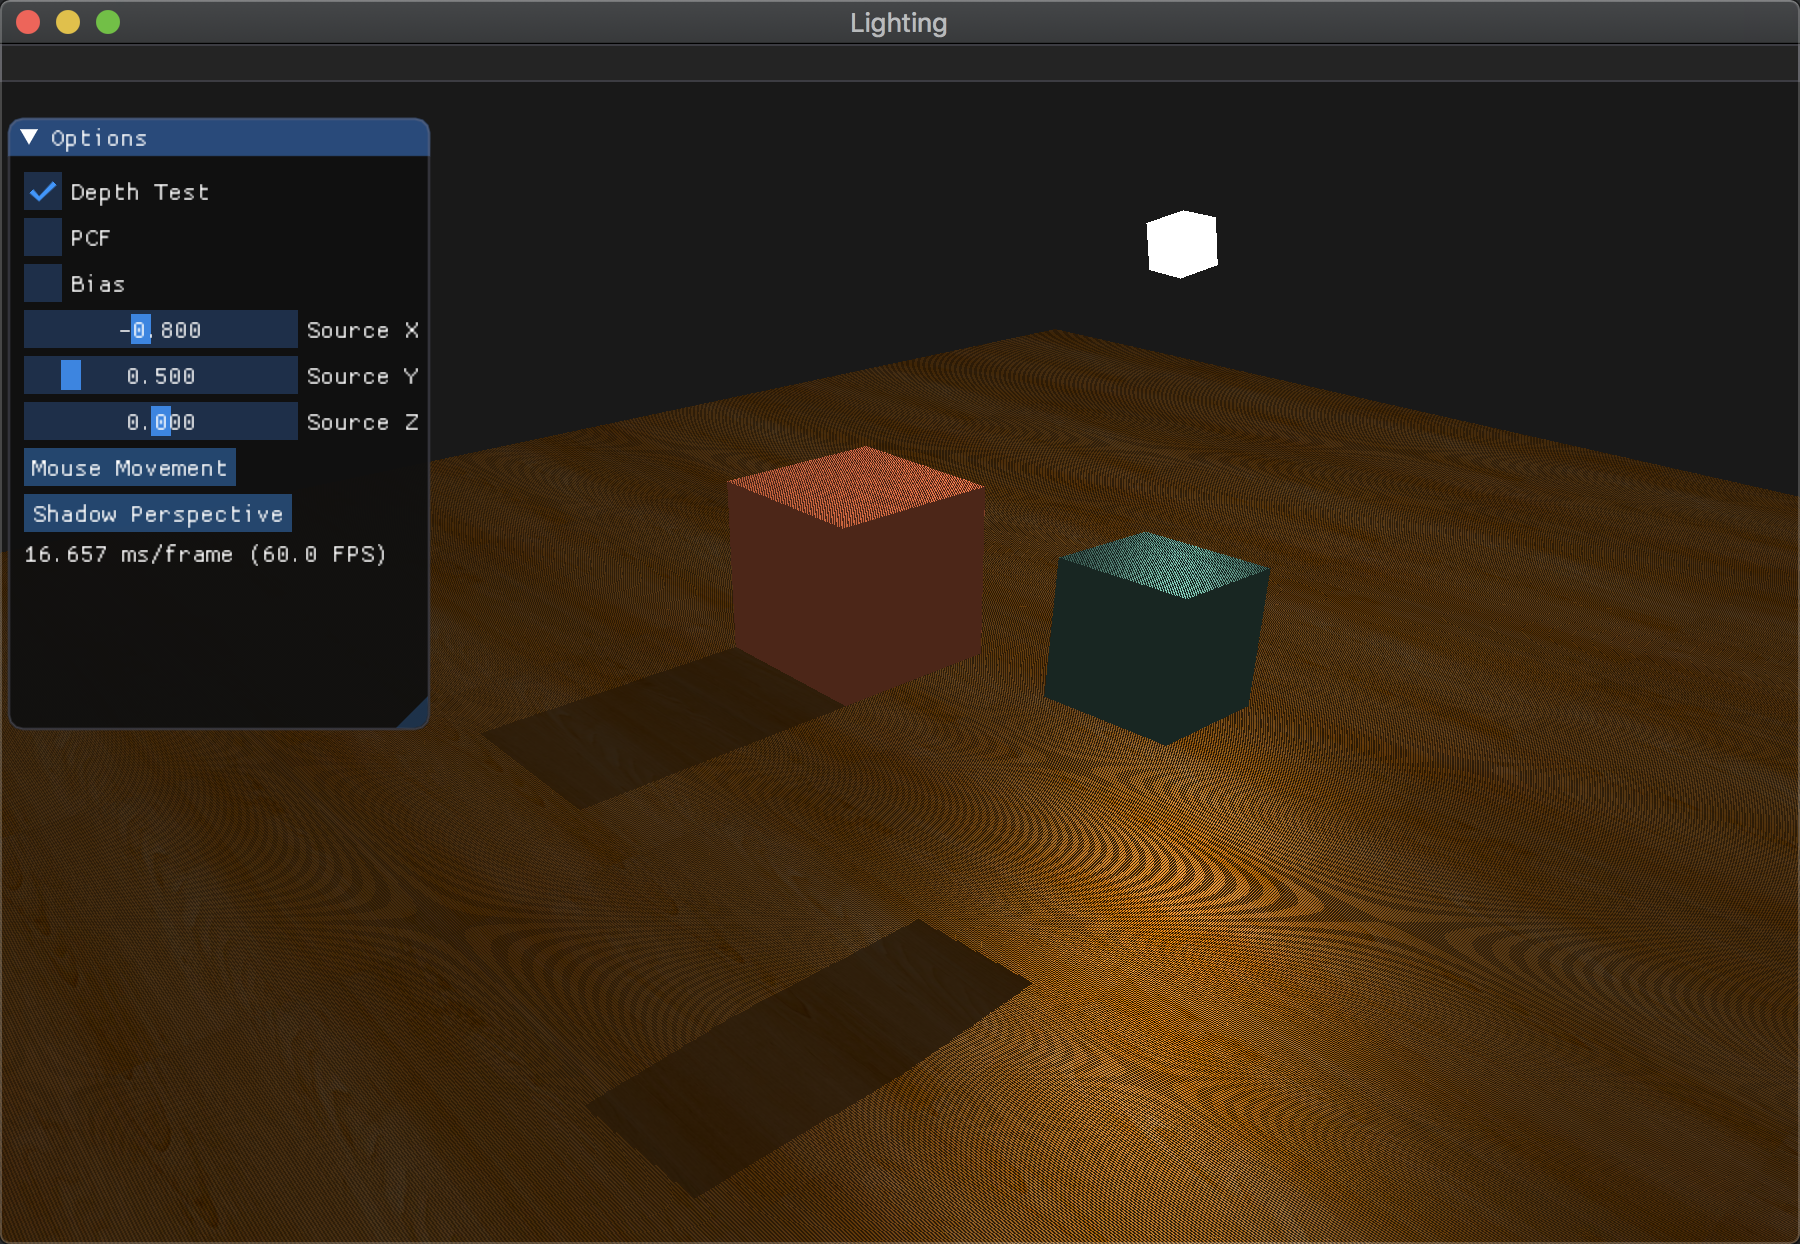
\includegraphics[scale=0.3]{1.png}
            \caption{阴影效果,白色 Cube 为光源,使用的投影为正交投影}
            \label{}
        \end{figure}

    \end{enumerate}
    
    \item 修改GUI
    
    修改 GUI 后可提供的功能有:
    \begin{enumerate}
        \item 开启或关闭深度测试
        \item 启动或关闭 PCF 消除锯齿
        \item 启动或关闭 bias 以消除阴影失真
        \item 调整光源位置
        \item 进入鼠标模式以通过鼠标调整摄像机方向
        \item 光源改为使用透视投影
    \end{enumerate}
    用户也可通过键盘 wasd 键输入控制摄像机位置。

    GUI 的效果如下:
    \begin{figure}[H]
        \centering
        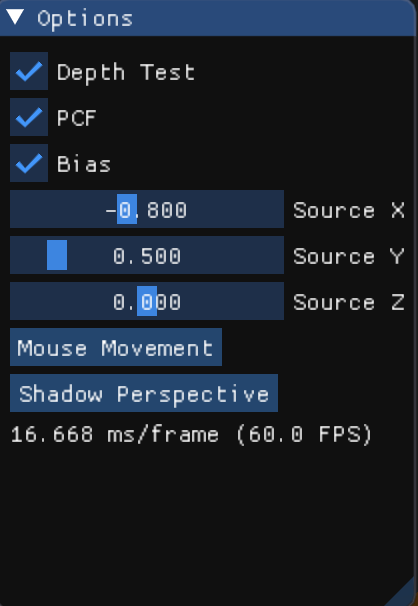
\includegraphics[scale=0.8]{gui.png}
        \caption{GUI}
        \label{}
    \end{figure}
\end{enumerate}

\section{Bonus}

\begin{enumerate}
    \item 优化Shadowing Mapping
    \begin{enumerate}
        \item 阴影失真
        
        上图可见实现的阴影效果会导致场景各处出现明显的线条状,即阴影失真,其出现原因如下图所示:

        \begin{figure}[H]
            \centering
            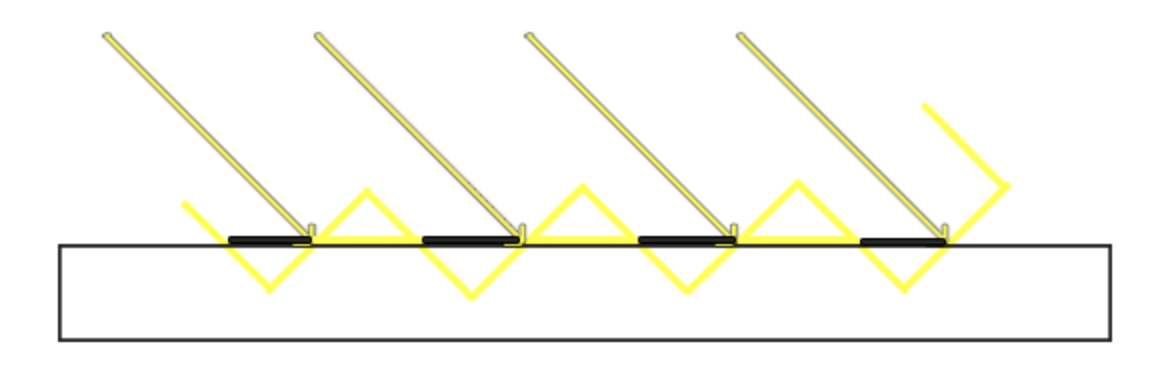
\includegraphics[scale=0.5]{acne.png}
            \caption{阴影失真}
            \label{}
        \end{figure}

        当光以一个角度射向表面时,多个片元会在一个斜坡的深度中采样,使得一部分像素的深度在表面之上,一部分在表面之下,从而导致条纹阴影的出现。

        一种解决方法是在表面深度上添加一个 Bias,如下图所示:
        \begin{figure}[H]
            \centering
            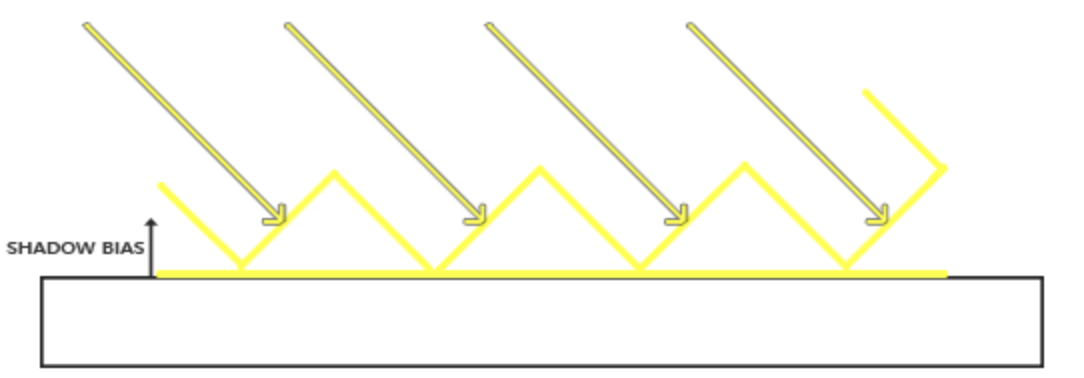
\includegraphics[scale=0.5]{bias.png}
            \caption{阴影偏移}
            \label{}
        \end{figure}
        其在片段着色器中的实现如下:
        \begin{lstlisting}
        float thetaCos = dot(normal, lightDir);
        float bias = 0;
        if (useBias) {
            bias = max(0.05 * (1.0 - thetaCos), 0.005);
        }
        shadow = currentDepth - bias > closeDepth  ? 1.0 : 0.0;
        \end{lstlisting}

        应用后效果如下,可见条纹状现象已去除:
        \begin{figure}[H]
            \centering
            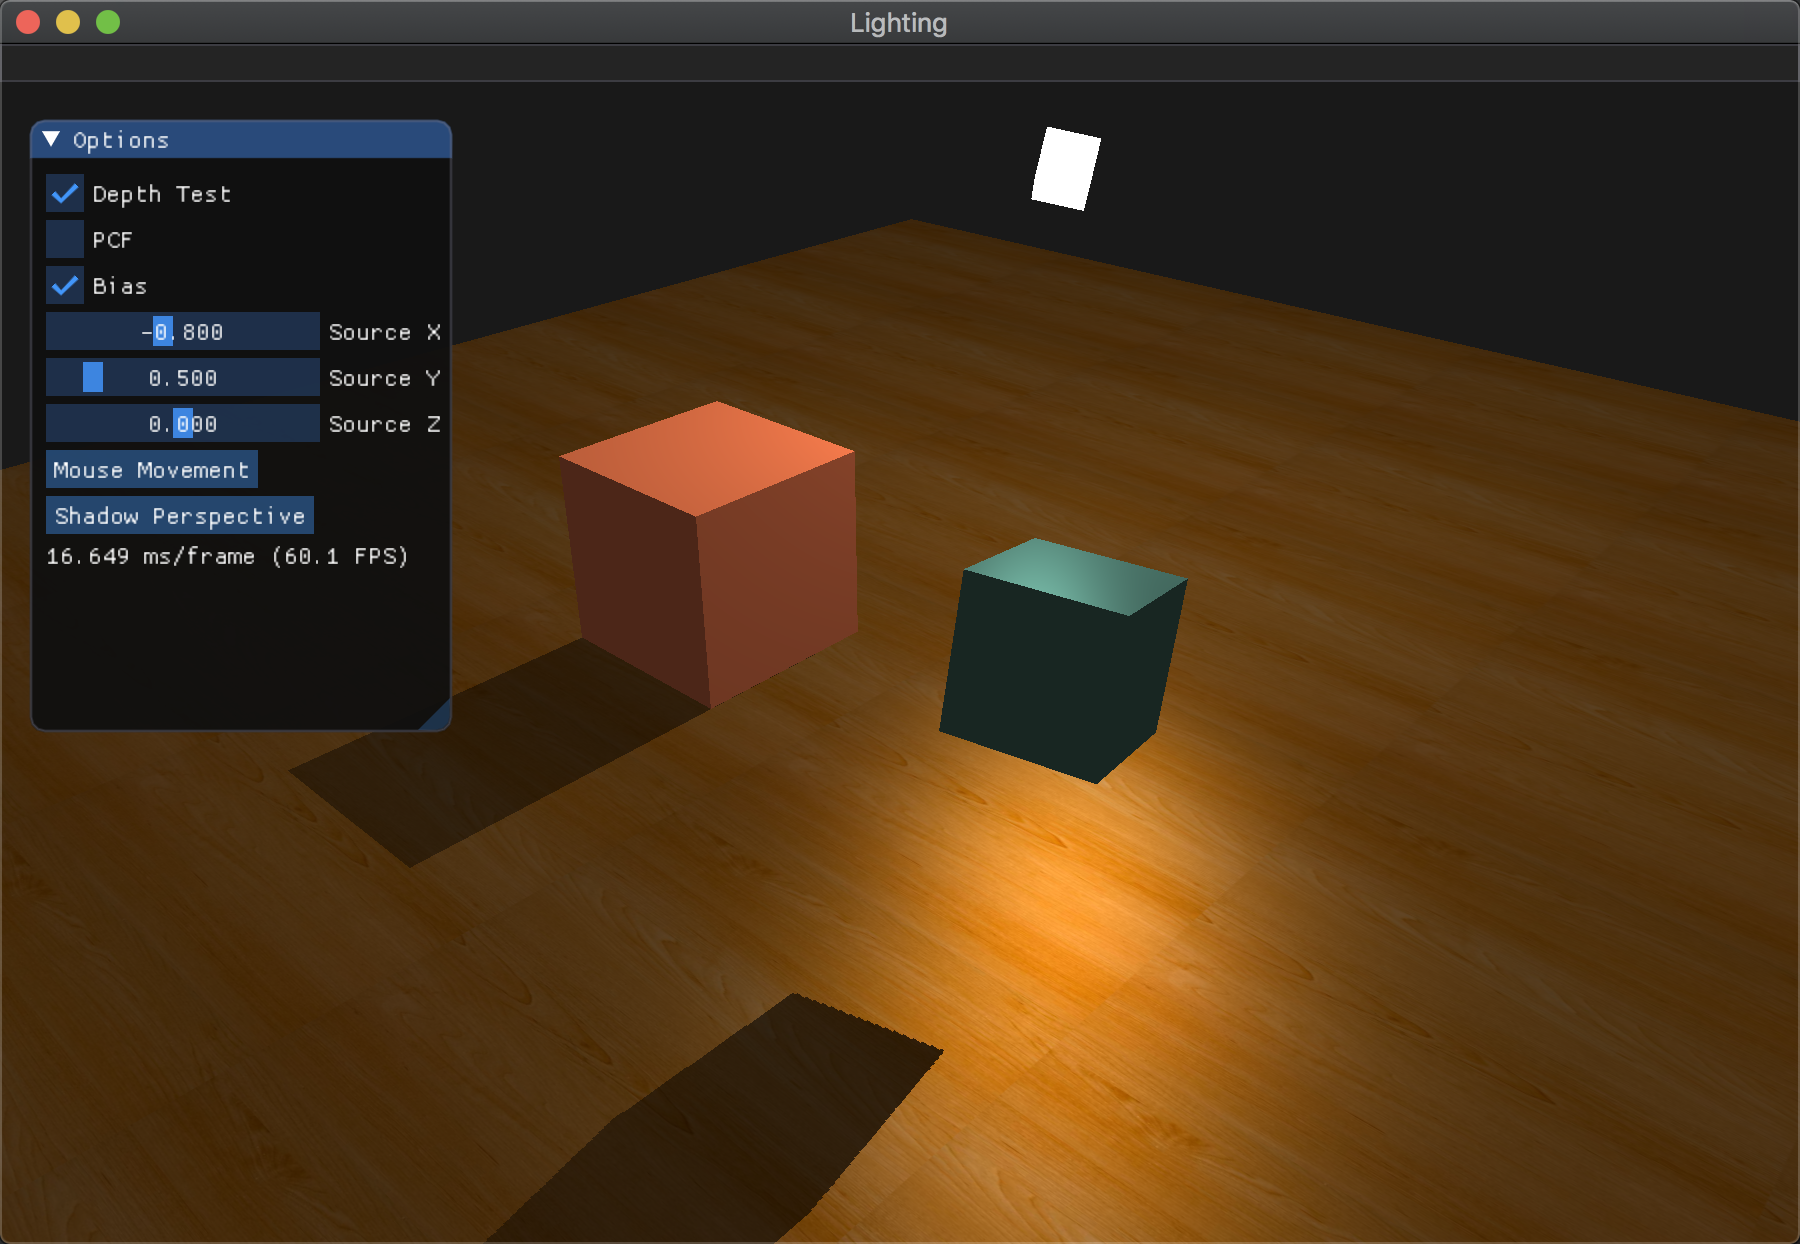
\includegraphics[scale=0.3]{bias-shadow.png}
            \caption{应用 Bias 后的阴影效果}
            \label{}
        \end{figure}

        \item PCF
        将摄像机移近阴影处,观察到阴影存在着许多锯齿:
        \begin{figure}[H]
            \centering
            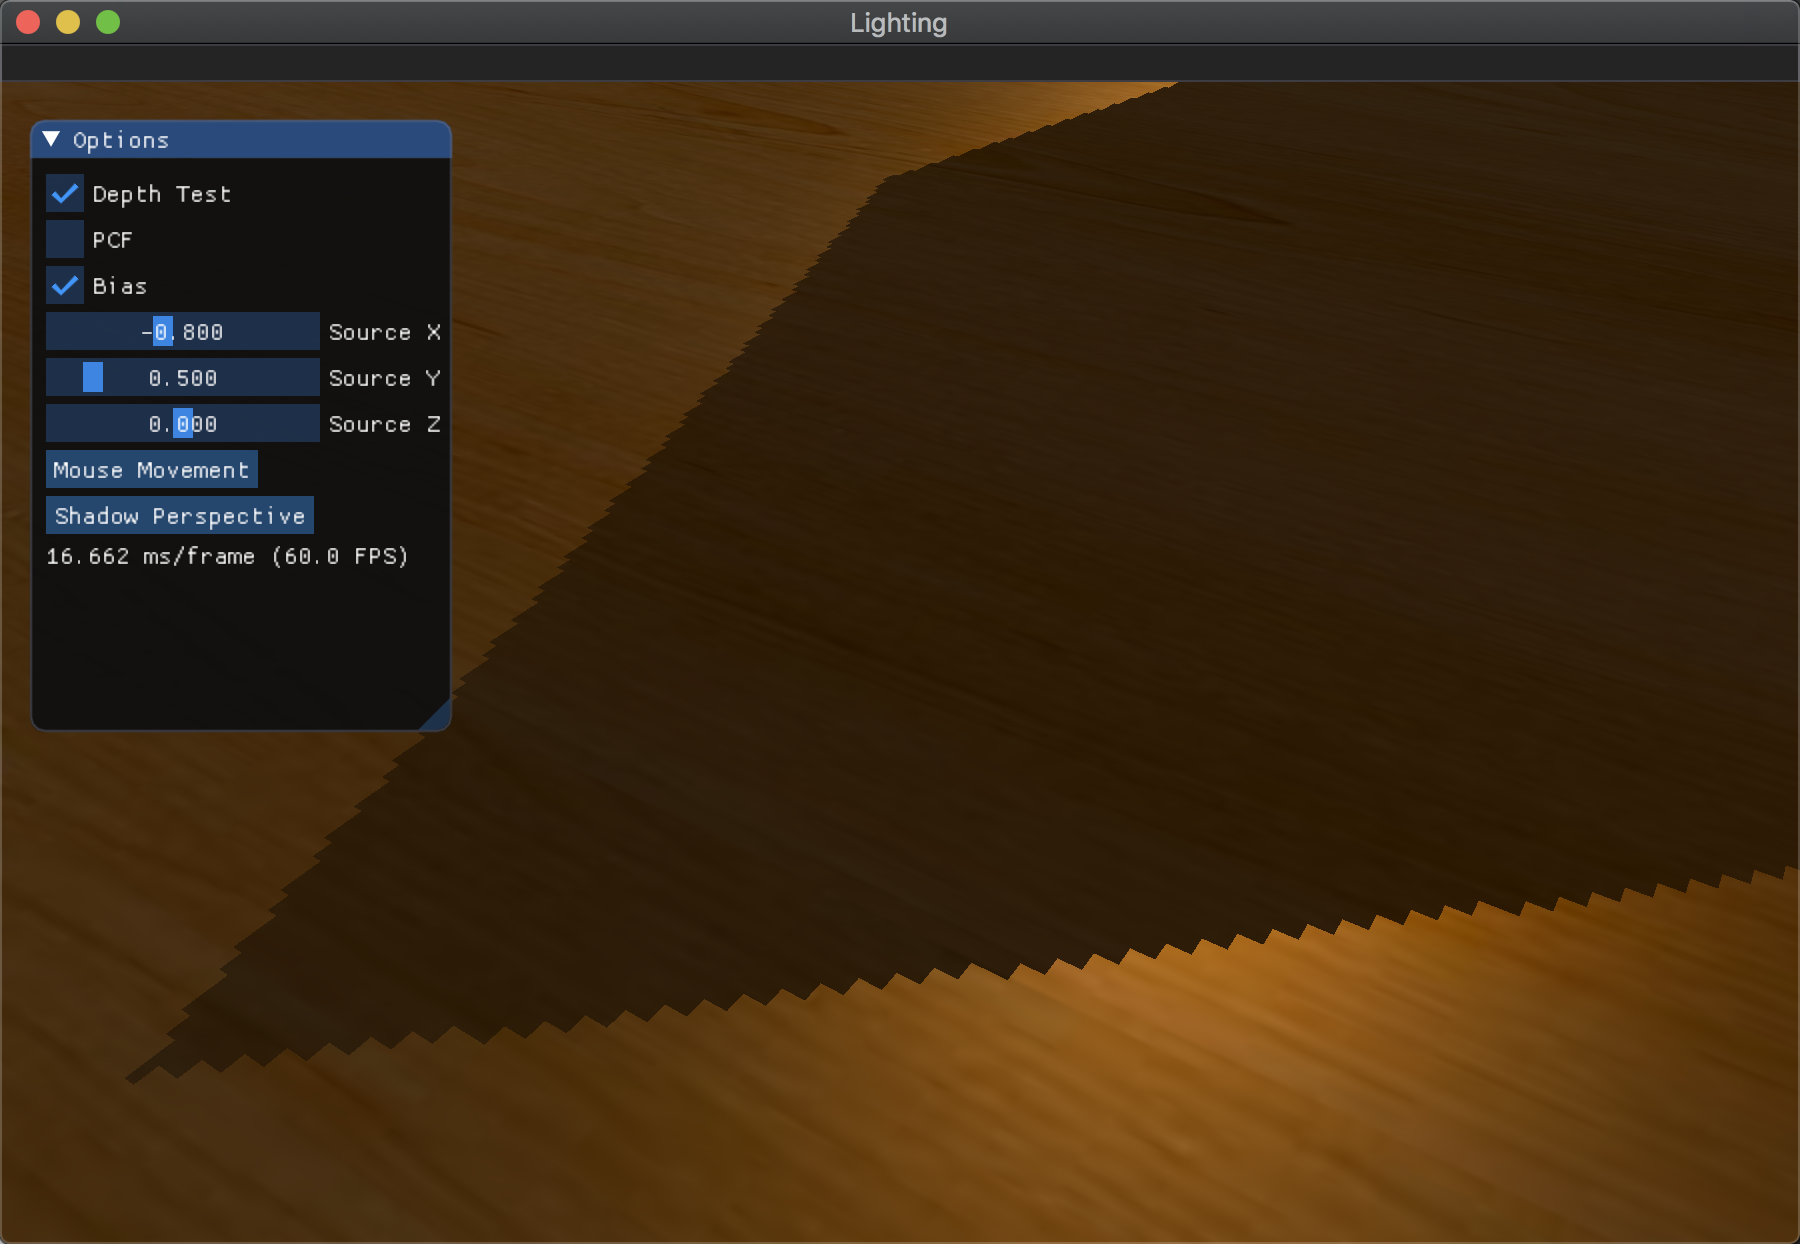
\includegraphics[scale=0.3]{alias.png}
            \caption{阴影锯齿}
            \label{}
        \end{figure}

        随着深度贴图解析度上升,锯齿的现象可以减少,在此之外的一种减少锯齿现象的方式是 PCF,其基本思路是对每一个点都对其周围点采样并取平均值为该点的阴影值。
        在片段着色器中的实现为:
        \begin{lstlisting}
        if (pcf) {
            vec2 texelSize = 1.0 / textureSize(shadowMap, 0);
            for (int x = -1; x <= 1; ++x) {
                for (int y = -1; y <= 1; ++y) {
                    float pcfDepth = texture(shadowMap, projCoords.xy + vec2(x, y) * texelSize).r;

                    shadow += currentDepth - bias > pcfDepth  ? 1.0 : 0.0;
                }
            }

            shadow /= 9.0f;
        }
        \end{lstlisting}

        应用后效果如下,可见较之未开启时,阴影锯齿更为柔和:
        \begin{figure}[H]
            \centering
            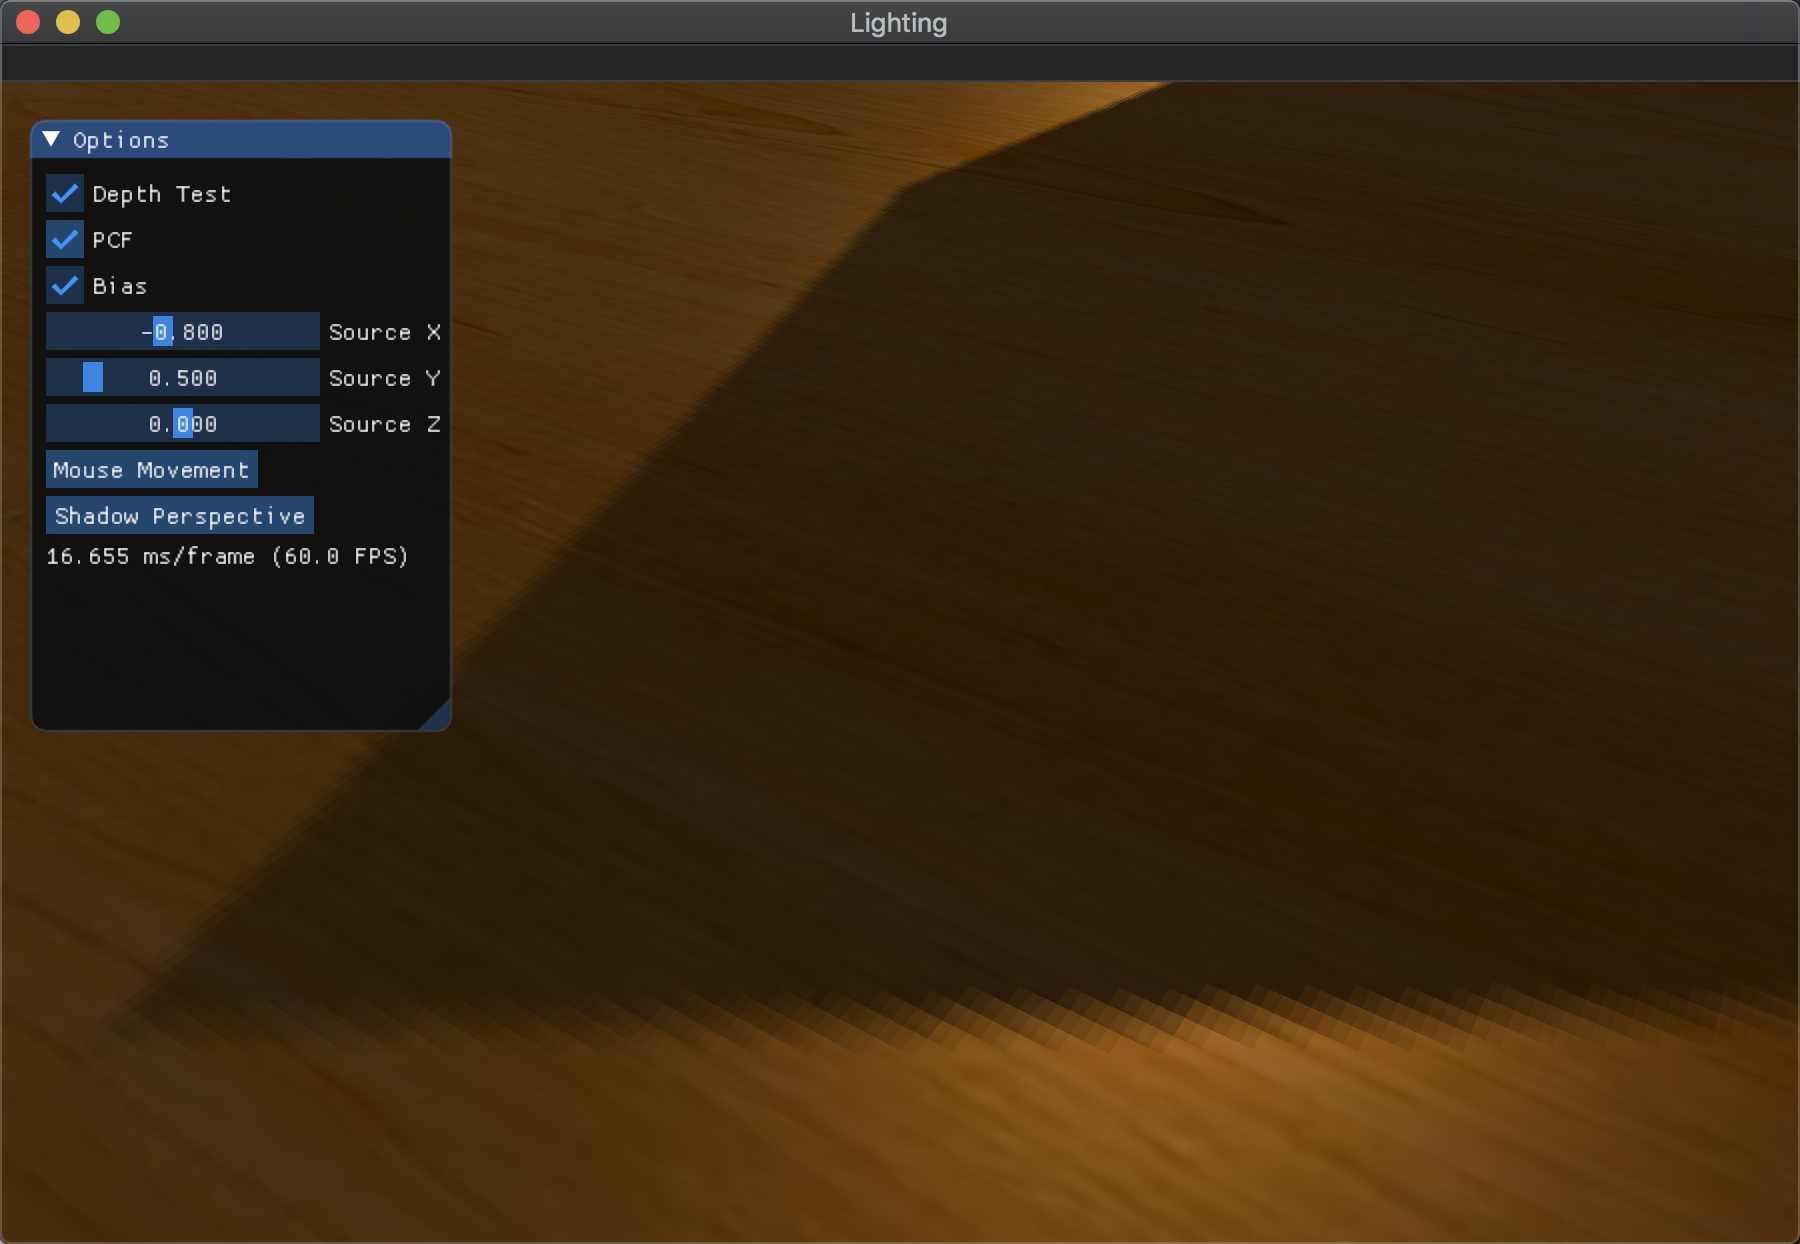
\includegraphics[scale=0.3]{pcf.png}
            \caption{开启 PCF 后效果}
            \label{}
        \end{figure}

    \end{enumerate}
    
\end{enumerate}




\end{document}
\grid
\grid
